\section{ANALYSIS AND RESULTS}

In order to study the socio-technical congruence hypothesis for the Cargo package manager, I started analysing its package dependency network and the associated technical and social (commenting) activities of its GitHub contributors.
To do so, I focused on the three preliminary research questions presented in Section~\ref{sec:intro}.


\textbf{RQ1 - } How does the dependency network structure influence social activity? (E.g., are contributors more likely to be active in commenting on packages they depend on than on other packages?) Here I want to talk about RQ1 %including whether the developer have had comment activity before start depeniding on a package, our findings there are less comment on packages with technical dependency than others but comments on packages which are dependent to each other are increasing as we move toward 2019. It seems that this tendency is going to grow more in recent years. Our investigation shows, the peak in Febraury 2016 caused by a major problem with 2 popular component which was led to a burst of comment by both users and contributors of those packages.

\textbf{RQ2 - } According to what I explained I am looking for any kind of evidence showing that if there is any kind of relationship between social activity of the contributors of packages and technical dependency of the packages. To do this in fact I basically tried to find a relation between any kind of social activity including issue comments, commit comment, pull review comment and pull comments of package maintainers and the dependency of each version of that package to find whether there is a tendency to put comment before start using a package or is there any behaviorial pattern between dependency network and social activity. If I can find any sign of action that shows its more likely for a developer to comment on package before start using it, based on this we can conclude social interaction can lead to technical dependency. My rudimental results shows that although not all activities will result in a technical dependency but there is priliminary evidence that shows there are a lot of cases that developer start using a package after commenting and to be more precise the result shows contributors tend to put comment on issues and pulls before depending on a package. the figure shows my finding in Cargo ecosystem.

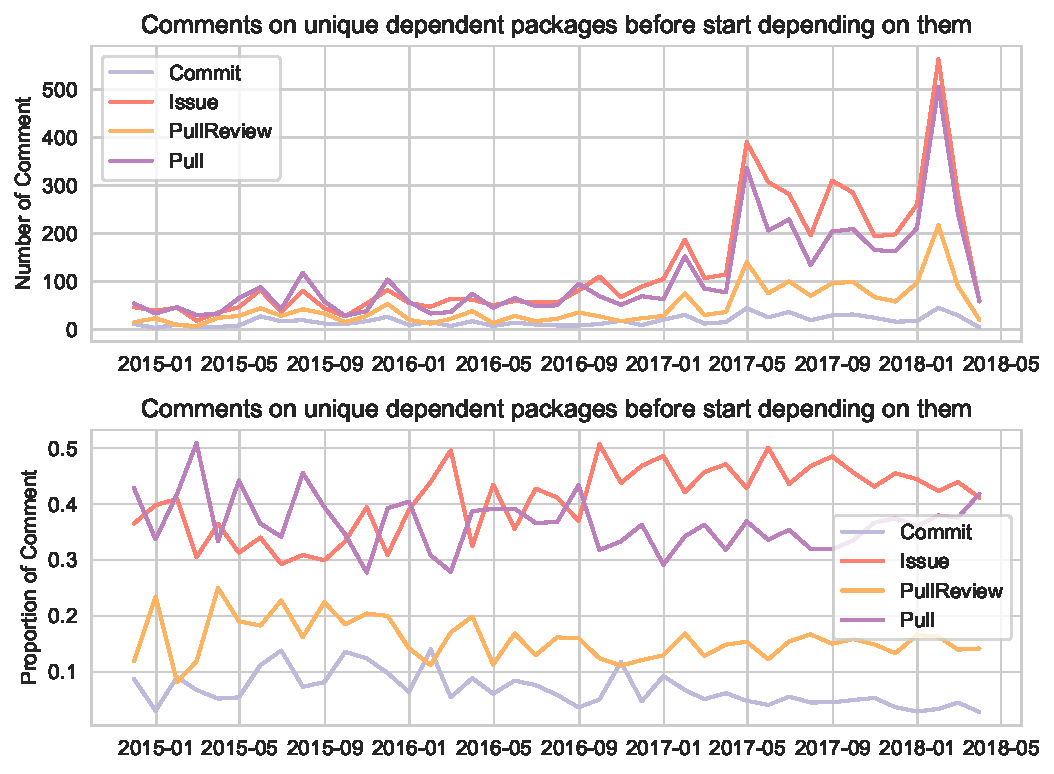
\includegraphics[width=\columnwidth]{Photos/RQ2.pdf} 


\textbf{RQ3 - } Here I want to talk about RQ1


